\documentclass[twocolumn,9]{ltjsarticle}

\usepackage[top=15mm,bottom=15mm,left=20mm,right=20mm]{geometry}
\usepackage[haranoaji,nfssonly]{luatexja-preset}
\usepackage{graphicx}
\usepackage{url}

\usepackage{multirow}    % セル結合用
\usepackage{tabularx}    % 表用&カラムサイズ指定
%% カラムサイズの指定用 %%
\newcolumntype{C}[1]{>{\centering\arraybackslash}p{#1}}
\newcolumntype{L}[1]{>{\raggedright\arraybackslash}p{#1}}
\newcolumntype{R}[1]{>{\raggedleft\arraybackslash}p{#1}}

\title{周期的な通信によるボットネット検出と対処優先度決定手法の提案}
\author{19FMI29 山下 尚彦 \\ 指導教員: 寺田 真敏}
\date{}

\begin{document}
\maketitle

\section{はじめに}
サイバー攻撃において, サーバやWebサイトに対して大量のアクセスを行いインターネットサービスをダウンさせる
DDoS攻撃というものがある. このDDoS攻撃は, マルウェアに感染した端末がボットネットと呼ばれる独自のネットワークを
構築し, それらの端末が攻撃命令を受けて一斉にアクセスすることで起こる. 
実際に2016年10月, DNSサービスを提供する会社を標的としたDDoS攻撃が行われた. 
これによりこの会社のDNSを利用していたオンラインサービスが影響を受け, 一時的にサービスを利用できない状態になり, 
被害額は1億1千万ドルと推定される. また, DDoS攻撃以外にもスパム/フィッシングメールの送信に
ボットネットが使われることもある. 

攻撃者はボットネットを用いる際にコマンド\&コントロールサーバ(C2サーバ)を通じて攻撃を命じる. 
また攻撃命令だけではなく, ボットネットに対して有効な状態であるかを確認するためにC2サーバは周期的に通信を行う. 
本研究ではボットネットとC2サーバ間の周期的な通信に着目し, ネットワーク上のボットネットを検出及び
C2サーバからのレスポンスによって対処の優先度を決定する手法を提案する. 

\section{関連研究}
Basilらの研究\cite{assadhan2018analysis}では, ボットネットとC2サーバ間の周期的な通信を検出する
手法を提案している. この研究では, 通信に用いられるプロトコルであるP2P, IRC, HTTPの規定のポート番号
11375, 6667, 80番ポート上の通信を監視し, 解析を行う. Basilらの実験ではP2PとIRCを用いたボットネットを
検出できたが, ボットネットによるHTTPを用いた通信はボットネット以外のアプリケーションの膨大な通信により
検出することができなかった. 

本研究では, Basilらの研究とは違い, ポート番号で通信をフィルタリングするのではなく, 送信元と受信先のIPアドレス毎に
通信をグループ分けすることで他のアプリケーションの通信による影響を受けにくし, さらにC2サーバからのレスポンスによって
ボットネットの対処優先度を決定することを目的とする. 

\section{提案手法}
本章ではボットネットとC2サーバ間の周期的な通信からボットネットを検出する手法と対処の優先度を決定する手法を提案する.
\subsection{周期性のある通信の検出方法}
提案手法では, 通信の周期性を推定するためにLomb-Scargleピリオドグラム\cite{vanderplas2018understanding}を用いた. 
このピリオドグラムは不定間隔, または欠損のある信号であっても周波数解析を行えるため, 
図\ref{fig:lombscargle}のような連続していない正弦波の周期性を推定することができる. 

\begin{figure}[htb]
    \centering
    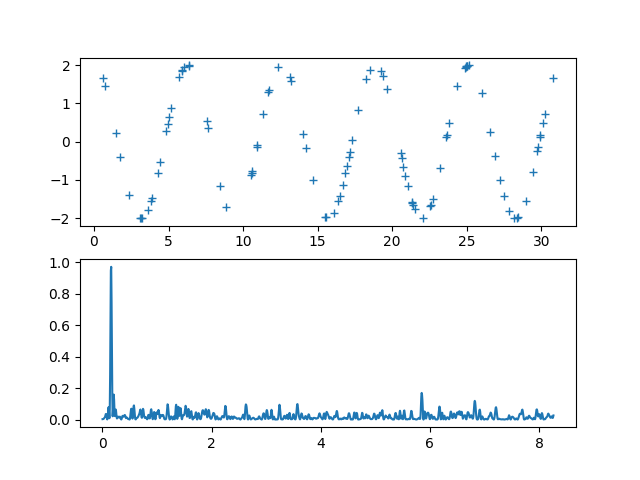
\includegraphics[width=8cm]{images/【実験】LombScargleピリオドグラムによるShinoBot通信の解析/lombscargle.png}
    \caption{欠損のある正弦波と解析結果}
    \label{fig:lombscargle}
\end{figure}

\subsection{周期性の測定方法}
Lomb-Scargleピリオドグラムによる信号の周期性はピークを用いることで判断することができる. 
これは, 信号が周期性のない正規分布だという過程に基づいてある一定の値以上のピークを解析結果が示した場合によって判断される. 
図\ref{fig:lombscargle}を例にすると, 図の正弦波が非周期的である確率が0.1\%以上, 
つまり99.9\%周期的であるためには, 図のグラフのピークが0.18631798(${=P_{0.1}}$)以上であることを意味する. 
このグラフのピークは0.9993959064009751と, ${P_{0.1}}$を超えているため99.9\%以上周期的であると言える. 

\subsection{対処優先度の決定方法}
ボットネットがC2サーバと通信を行った際に, C2サーバからHTTPレスポンスステータスコードが返送される. 
これはHTTP通信においてリクエストが正常に完了したかどうかを示す3桁の数字からなるコードで, 
主に200-299, 400-499, 500-599が使われる. 200番台はリクエストが正常に完了したことを表し, 
400番台はURLの間違いによってサーバがリソースを発見できなかったことを示す404(Not Found)などの
クライアントによるエラー, 500番台はサーバ側で処理できない事態が発生した500(Internal Server Error)などの
サーバ側で起きるエラーを示す. 

本研究では, このHTTPレスポンスステータスコードに着目してボットネットの対処優先度を決定する. 
前節で示した方法で周期性のあるIPアドレスのペアのステータスコードを調べて200番台であれば緊急性のある事案とし, 
400番台の場合は, C2サーバは稼働している可能性があるがボットネット側のエラーによってリクエストが正常に完了していない
ことがわかるので, 200番台ほどではないが対処する必要がある事案とする. さらに400番台の中でのステータスコードによって
エラーの種類がわかるため, 更に細かく優先度を設定することができると考えられる. 
500番台に関してはC2サーバ側でエラーが発生しているため優先度を低くすることができる. 

\section{実験}
\subsection{実験データ}
今回の実験で使用するBOS2016は, 総務省実証事業「サイバー攻撃解析・防御モデル実践演習の実証実験の請負」にて実施し, 
研究者コミュニティから提供された組織内ネットワークへの侵害活動を観測されたデータセット\cite{マルウェア対策研42:online}
であり, マルウェア検体のハッシュ値情報や, 通信観測データ, プロセス観測データの他に, Windowsのイベントログや
ファイアウォールのログのデータを保持している. 
マルウェアの検体は以下の表\ref{tab:bos2016}からわかるように, 動作が確認され通信が発生し, 攻撃の観測ができたものから, 
動作が確認されC2サーバへのSYNパケットのみが送信された検体, C2サーバとの通信を確認できなかったもの, 
検体の実行ができず通信が発生しなかったものがある. 

\begin{table}[htb]
    \centering
    \caption{BOS2016の検体の挙動と通信について}

    \begin{tabular}{C{2cm}L{1.5cm}L{2.8cm}}
        %% カラム名 %%
        \hline
        観測データ\par ディレクトリ & 挙動 & 通信 \\
        \hline \hline
        %% データ %%
        e04 & 動作 & 攻撃活動を観測 \\ \hline
        e12\par e20 & 動作 & C2サーバとの通信が成立しない(403, 404, 503) \\ \hline
        e43 & 実行不可 & 通信発生せず \\ \hline
        e70\par e435 & 動作 & C2サーバへSYNパケットのみ送信 \\
        \hline
    \end{tabular}
    \label{tab:bos2016}
\end{table}

\subsection{解析手順}
まず, ネットワーク上の通信を観測したファイル(PCAPファイル)から以下の情報を抽出して,
解析に不要な情報を排除する. 

\begin{itemize}
    \item 通信時間のタイムスタンプ
    \item 送信元IPアドレス
    \item 受信先IPアドレス
\end{itemize}

次に,送信元IPアドレスと受信先IPアドレスのペアになるように通信データを分け, 
Lomb-Scargleピリオドグラムで周波数解析を行う. 

\section{結果}
以下の表\ref{tab:result}は, e12, e20, e43, e70, e435それぞれの
送信IPアドレス数(表\ref{tab:result}のsrc), 
送信元と受信先IPアドレスのペア数(表\ref{tab:result}のpair), 
通信が周期的でない確率が0.5\%以下のペア数(表\ref{tab:result}の${P_{0.5}}$), 
通信が周期的でない確率が0.1\%以下のペア数(表\ref{tab:result}の${P_{0.1}}$), 
通信が周期的でない確率が0.01\%以下のペア数(表\ref{tab:result}の${P_{0.01}}$)
をまとめた表である.  \\
eXXはe12, e20, e43, e70を, eXXXはe435で実行した検体の通信を含めた全体のネットワークを観測したデータである. 
実験の結果, 全体のペア数と比べて${P_{0.01}}$のペア数は8分の1以下に絞り込むことができた. 

\begin{table}[htb]
    \centering
    \caption{BOS2016の実験結果}

    \begin{tabular}{C{8mm}L{8mm}L{8mm}L{8mm}L{8mm}L{8mm}L{8mm}}
        %% カラム名 %%
        \hline
        {} & src & pair & ${P_{0.5}}$ & ${P_{0.1}}$ & ${P_{0.01}}$ \\
        \hline \hline
        %% データ %%
        eXX  & 410 & 1183 & 152 & 94 & 65 \\
        e12  & 32  & 63   & 0   & 0  & 0  \\
        e20  & 12  & 23   & 0   & 0  & 0  \\
        e43  & 22  & 42   & 2   & 2  & 1  \\
        e70  & 24  & 49   & 11  & 10 & 6  \\
        eXXX & 217 & 550  & 107 & 73 & 57 \\
        e435 & 20  & 39   & 1   & 1  & 1  \\
        \hline
    \end{tabular}
    \label{tab:result}
\end{table}

\section{今後の予定}
今回の実験ではボットネットとC2サーバの定期的な通信を絞り込むことができたが, HTTPレスポンスステータスコードによる
対処優先度を決定する段階まで至らなかったため, 今後は優先度を決定する手法に力を入れたいと思う. 
そのために, C2サーバが返送するレスポンスデータについて調査したり, スターテスコードによってどのように優先度を決定するか
などの評価の部分を考える必要がある. 

\bibliographystyle{junsrt}
\bibliography{DB}
\end{document}